\begin{figure}[htbp]
\centering
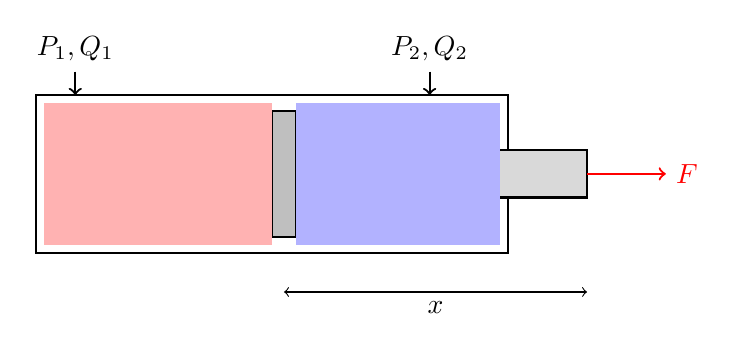
\begin{tikzpicture}
    % Cylinder
    \draw[thick] (0,0) rectangle (6,2);

    % Piston
    \draw[thick, fill=gray!50] (3,0.2) rectangle (3.3,1.8);

    % Rod
    \draw[thick, fill=gray!30] (3.3,0.7) rectangle (7,1.3);

    % Chambers
    \fill[red!30] (0.1,0.1) rectangle (3,1.9);
    \fill[blue!30] (3.3,0.1) rectangle (5.9,1.9);

    % Ports
    \draw[->, thick] (0.5,2.3) -- (0.5,2) node[above, pos=0] {$P_1, Q_1$};
    \draw[->, thick] (5,2.3) -- (5,2) node[above, pos=0] {$P_2, Q_2$};

    % Displacement
    \draw[<->] (3.15,-0.5) -- (7,-0.5) node[midway, below] {$x$};

    % Force
    \draw[->, thick, red] (7,1) -- (8,1) node[right] {$F$};
\end{tikzpicture}
\caption{Double-acting hydraulic cylinder.}
\label{fig:hydraulic_cylinder}
\end{figure}
